% A workaround to allow relative paths in included subfiles
% that are to be compiled separately
% See https://tex.stackexchange.com/questions/153312/subfiles-inside-a-subfile-using-relative-paths
\providecommand{\main}{..}
\documentclass[\main/thesis.tex]{subfiles}

\begin{document}

\chapter{Introduction}

\section{Motivation}
\subsection{Background}
Many datasets can be represented by networks consisting of a set of nodes and edges connecting these edges. Examples include protein-protein interaction networks \cite{krogan2006global}, food webs \cite{williams2000simple}, social networks \cite{shetty2004enron}, air transportation networks, collaboration networks \cite{nascimento2003analysis,leskovec2007graph} and the worldwide web \cite{albert1999internet,broder2000graph}. The study of networked systems has a history stretching back several centuries. Because of its broad applications in different domains, network analysis has attracted increasing attention from computer scientists, biologists and physicists recently. There are a lot of interesting research topics in complex network analysis. Among them, the problems such as link prediction, community detection and entity ranking have received a considerable amount of attention.

\subsubsection{Link Prediction}
Link prediction is the problem of determining future or missing associations between entities in complex networks based on observed links. It can be categorized into two classes: one is forecasting the future links, which can be used to help on-line social network users find new friends; the other is determining the hidden or unobserved relationships between nodes, such as protein-protein interaction networks and food webs. The discovery of interaction links in biological networks is usually expensive, therefore, finding the most promising latent links instead of checking all possible links is important in reducing experimental costs.

In the past decade, many works have been done about link prediction in certain graphs, graphs where the network structure is exactly and deterministically known. There are many metrics available for computing the similarity of two nodes. According to the characteristics of these metrics, they can be divided into neighbor-based metrics, path-based metrics, random-walk-based metrics and social theory-based metrics. Furthermore, there are some learning-based methods that have been proposed in recent years.

Among all approaches, neighbor-based metrics are effective and the simplest way to predict missing links. These metrics assume that two nodes are more likely to be connected if they have more common neighbors. Common Neighbors (CN) \cite{newman2001clustering} is the simplest metric among all neighbor-based metrics. It simply counts the number of common neighbors between two nodes and ignores their total number of neighbors. To improve the prediction accuracy, some variants such as Salton Index \cite{salton1986introduction} and Jaccard Index \cite{jaccard1901etude} are also used in link prediction. They improve link prediction accuracy by taking the number of neighbors that the two nodes have into account. CN also ignores that different common neighbors have different contributions on the connection likelihood. To solve this problem, other variants such as Adamic-Adar (AA) Index \cite{adamic2003friends} and Resource Allocation (RA) Index \cite{zhou2009predicting} are proposed, where a common neighbor with low degree is advocated for by assigning more weight to it.

\subsubsection{Community Detection}
The nodes in many networks fall naturally into groups or communities. Nodes in the same community are densely connected, while the number of edges between nodes of different communities is much smaller. Community detection is the problem of finding such communities in complex networks based on edges between nodes. Detection of these communities is key to understanding the structure of complex networks and extracting useful information from them. The discovery of communities in networks can be useful in various applications. For example, detection of groups within the worldwide web can be used to find sets of web pages on related topics \cite{flake2002self}; detection of groups within social networks can also be used to find social units or communities \cite{girvan2002community}. Besides, community detection can also be used in analyzing trend in citation networks \cite{bedi2016community} and improving recommender systems \cite{cao2015improved}. 

In the past 15 years, a large number of community detection detection algorithms have been proposed for certain graphs, graphs where the network structure is exactly and deterministically known. According to the characteristics of these algorithms, they can be divided into graph partitioning-based algorithms \cite{kernighan1970efficient,newman2013community}, clustering-based algorithms \cite{girvan2002community,newman2004fast,blondel2008fast,clauset2004finding}, genetic algorithms (GA)-based algorithms \cite{pizzuti2008ga} and label propagation-based algorithms \cite{raghavan2007near}.

\subsubsection{Entity Ranking}
Entity ranking is the task of ordering sets of objects within the network based on the relations among them and the overall linking structure. Ranking nodes in networks can be useful in many applications. For example, in the context of web information retrieval, entity ranking methods can be used to rank webpages. (Needs more examples) To identify the most important nodes in a network, many centrality measures are proposed, such as degree centrality, closeness centrality \cite{freeman1978centrality}, betweenness centrality \cite{freeman1977set}, eigenvector Centrality \cite{bonacich1987power} and pagerank centrality \cite{page1999pagerank}.

\subsection{Challenges}
Most previous studies on complex network analysis have focused on networks under where the structure is exactly known. With the increasing number of applications in which the edges  are  constructed  in  the  network  through  uncertain  or statistical  inference,  the  problem  of  complex network analysis with edge uncertainty has become increasingly important. Examples of such networks  include  protein-protein  interaction  networks  with experimentally inferred links, sensor networks with  uncertain  connectivity  links,  or  social  networks, which are augmented with inferred friendship, similarity, or trust links. However, only few studies take probabilities into consideration. 

For the link prediction problem, Ahmed \cite{ahmed2016efficient} proposed the uncertain version of the random walk method for link prediction with edge uncertainty. Mallek \cite{mallek2016evidential} put forward an approach combined sampling techniques and information fusion and obtained good results in real-life settings. Up to now, the uncertain version of the popular neighbor-based metrics have not been studied. Murata and Moriyasu \cite{murata2007link} proposed three weighted similarity indices, including variants of the Common Neighbors, Adamic-Adar and Preferential Attachment indices, respectively. People may regard probabilities as weights and apply weighted variants of those metrics; however, it may lead to some problems. More details can be found in Section 4.

For the task of community detection, to solve the uncertain problem, Krogan \cite{krogan2006global} converted the uncertain network into a conventional binary network by thresholding the likelihoods. Johan \cite{dahlin2011method} proposed a method which is based on sampling from an ensemble of certain networks that are consistent with the available information about the uncertain networks. Lin \cite{liureliable} developed a novel k-means algorithm to solve the uncertain clustering problem. Travis \cite{martin2016structural} gave a principled maximum-likelihood method for inferring community structure. However, another issue exists in these algorithms is that they require knowledge of the entire graph structure to identify communities. The requirement of accessing the whole network information can not be satisfied when networks become too large to know completely, e.g., the WWW. In this scenario, it is hard to identify global communities, however, finding local community for a certain node is still useful. A local community is a community defined based on local information without having access to the entire network. For instance, we may want to quantify local community of a person given his social network in Facebook. Though the problem of local community detection on certain graphs have been discussed by some researchers, and several different local modularity metrics \cite{clauset2005finding,chen2009detecting,chen2009local} have been proposed to identify local community structure given limited information. The problem of local community detection on uncertain graphs is not yet solved.

For the problem of entity ranking in uncertain networks, Sevon et al. \cite{sevon2006link} proposed to transform the probabilities into weights by taking the negative logarithm of the probabilities. Then standard algorithms for finding shortest paths can be applied. Closeness centrality and betweenness centrality can also be calculated based on shortest paths. Pfeiffer and Neville \cite{pfeiffer2010probabilistic} formulated a measure of centrality based on the most probable paths of communication, rather than shortest paths. They developed a notion of probabilistic paths in uncertain networks, and used it as a foundation for computing probabilistic betweenness centrality in uncertain networks. A major shortcoming of both methods is that they can only be applied to unweighted probabilistic graphs. For weighted probabilistic graph, ignoring the original weights of the graph could cause the two methods to perform badly.
% Many datasets can be represented by networks consisting of a set of nodes and edges connecting these edges (mix from Jiyang, Newman and review paper). Examples include protein-protein interaction networks \cite{krogan2006global}, food webs \cite{williams2000simple}, social networks \cite{shetty2004enron}, air transportation networks, collaboration networks \cite{nascimento2003analysis,leskovec2007graph} and the worldwide web \cite{albert1999internet,broder2000graph}(add citations, check Jiyang) (write by myself). The nodes in many networks fall naturally into groups or communities. Nodes in the same community are densely connected, while the number of edges between nodes of different communities is much smaller (from Newman, changed). Community detection is the problem of finding such communities in complex networks based on edges between nodes. Detection of these communities is key to understanding the structure of complex networks and extracting useful information from them. The discovery of communities in networks can be useful in various applications (from review paper). For example, detection of groups within the worldwide web can be used to find sets of web pages on related topics \cite{flake2002self}(citation, check Newman); detection of groups within social networks can also be used to find social units or communities \cite{girvan2002community}(citation, check Newman) (from Newman, changed). Besides, community detection can also be used in analyzing trend in citation networks \cite{bedi2016community}(citation) and improving recommender systems \cite{cao2015improved} (citation) (check review, last page). Because of its broad applications in different domains, link prediction has attracted increasing attention from computer scientists, biologists and physicists recently. 

%Most previous approaches on community detection have focused on networks where the structure is exactly known, and they require knowledge of the entire graph structure to identify communities. When we run these algorithms. we need to access and see the whole network information. However, recently we are faced with two problems. The first problem is that we have increasing number of networks which have edge uncertainty, which means the network structure is not exactly and deterministically known. The edges are constructed through uncertain or statistical inference, so we only know the connections between nodes with a certain probability. Examples of such networks include protein-protein interaction networks with experimentally inferred links, sensor networks with uncertain connectivity links, or social networks, which are augmented with inferred friendship, similarity, or trust links. Another problem of previous methods is that the requirement of accessing the whole network information can not be satisfied when networks become too large to know completely, e.g., the WWW. In this scenario, it is hard to identify global communities, however, finding local community for a certain node is still useful. A local community is a community defined based on local information without having access to the entire network. For instance, we may want to quantify local community of a person given his social network in Facebook.

% Most previous approaches on community detection have focused on networks where the structure is exactly known, and they require knowledge of the entire graph structure to identify communities. When we run these algorithms. we need to access and see the whole network information. (Jiyang, changed) However, recently we are faced with two problems. The first problem is that we have increasing number of networks which have edge uncertainty, which means the network structure is not exactly and deterministically known. The edges are constructed through uncertain or statistical inference, so we only know the connections between nodes with a certain probability. Examples of such networks include protein-protein interaction  networks with experimentally inferred links, sensor networks with uncertain  connectivity  links, or social networks, which are augmented with inferred friendship, similarity, or trust links. Another problem of previous methods is that the requirement of accessing the whole network information can not be satisfied when networks become too large to know completely, e.g., the WWW. (myself, based on Jiyang) In this scenario, (people may only want to know the local community for a certain node) it is hard to identify global communities, however, finding local community for a certain node is still useful. A local community is a community defined based on local information without having access to the entire network. For instance, we may want to quantify local community of a person given his social network in Facebook.
%NEEDS AT DEFINITION OF LOCAL COMMUNITY DETECTION AT SOME WHERE.

%To solve the first problem, Krogan \cite{krogan2006global} converted the uncertain network into a conventional binary network by thresholding the likelihoods. Johan \cite{dahlin2011method} proposed a method which is based on sampling from an ensemble of certain networks that are consistent with the available information about the uncertain networks. Lin \cite{liureliable} developed a novel k-means algorithm to solve the uncertain clustering problem. Travis \cite{martin2016structural} gave a principled maximum-likelihood method for inferring community structure. To solve the second problem, several different local modularity metrics \cite{clauset2005finding,chen2009detecting,chen2009local} have been proposed to identify local community structure given limited information. These methods aimed to solve one of the two aforementioned problems. However, the two problems may appear simultaneously in some scenarios. Up to now, there is no algorithm which is able to tackle both problems at the same time.


\section{Problem Definition}
\subsection{Networks with Edge Uncertainty}
An uncertain graph $\mathcal{G = (V,E,P)}$ is defined over a set of nodes $\mathcal{V}$, a set of edges $\mathcal{E}$, and a set of probabilities $\mathcal{P}$ of edge existence. Note the probability over the edge between node $\mathcal{V}_i$ and node $\mathcal{V}_j$ can be represented as $\mathcal{P}_{i,j}$ or $\mathcal{P}_{j,i}$. The multiple links and self-connections are not allowed. Figure \ref{uncertain_network_example} is an example of an uncertain network.
\begin{figure}
\centering
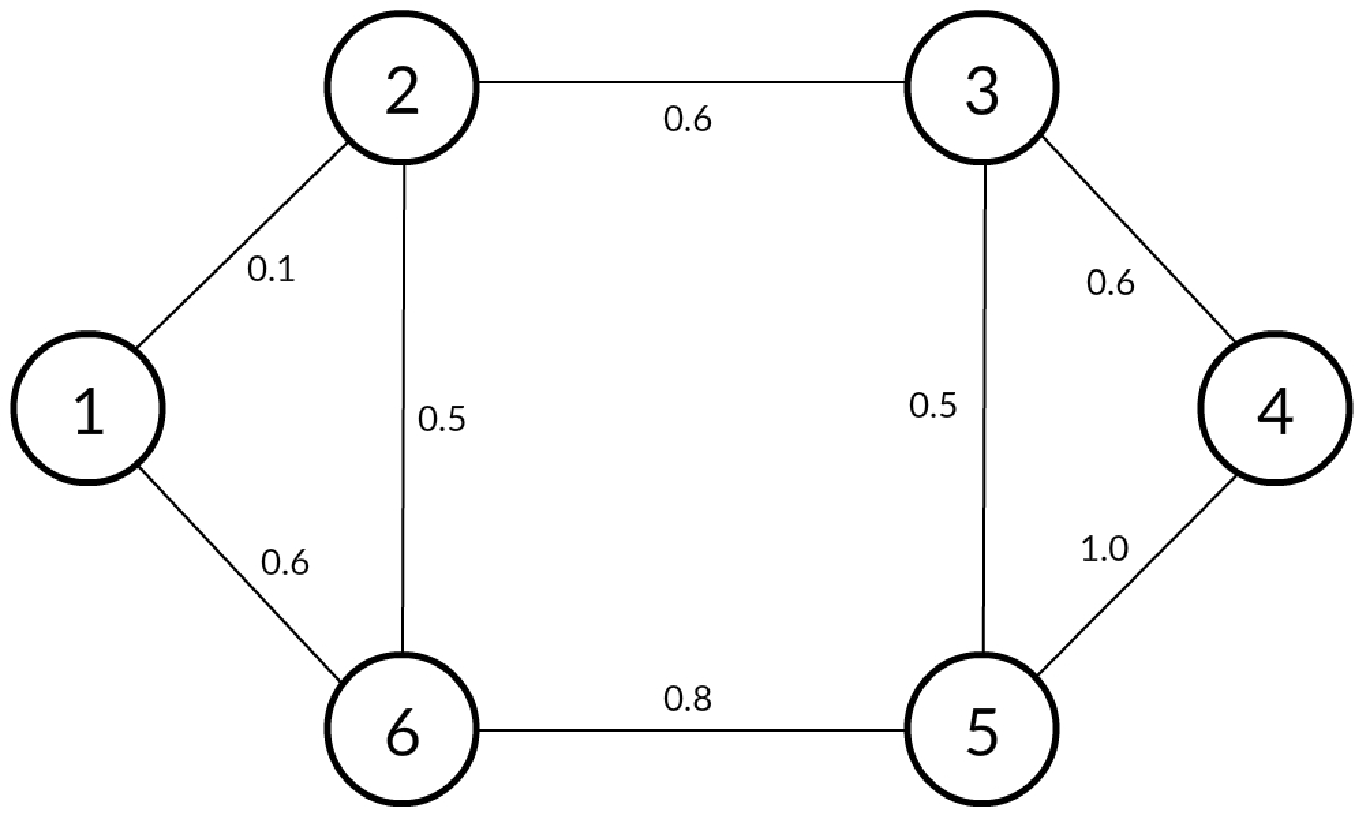
\includegraphics[scale = 0.35]{\main/img/probabilistic_graph.pdf}
\caption{An example of uncertain network. The numbers are existential probabilities.}
\label{uncertain_network_example}
\end{figure}

\subsection{Link Prediction for Uncertain Networks}
The task of link prediction is to discover future or missing associations between two nodes. To do this, for each pair of nodes, $\mathcal{V}_x,\mathcal{V}_y\in \mathcal{V}$, which are not directly connected, we assign a score, $s_{xy}$, according to a given similarity measure. A higher score means nodes $\mathcal{V}_x$ and $\mathcal{V}_y$ are more likely to have an edge. All the nonexistent links are sorted in a descending order according to their scores, and the links at the top are most likely to exist.

Generally, we do not know which links are the missing or future links, otherwise we do not need to do predictions. Therefore, to evaluate algorithms, we use known networks, hide some links, use link prediction algorithms to predict those hidden links and compare the prediction results. Based on the type of network, the observed edges $E$ can be divided into training set $E^T$ and probe set $E^P$ randomly or according to the timestamp. If the known network is time-varying and we know the time each change happens, we can regard the network before a certain time as the training set and the remaining as the probe set. Otherwise, we can just divide the training set and the probe set randomly. To quantify the accuracy of prediction algorithms, we use Precision as our evaluation metric. Figure 2 shows the overall procedures for our experiments. More experiment details can be found in Section 5.
\begin{figure}
\centering
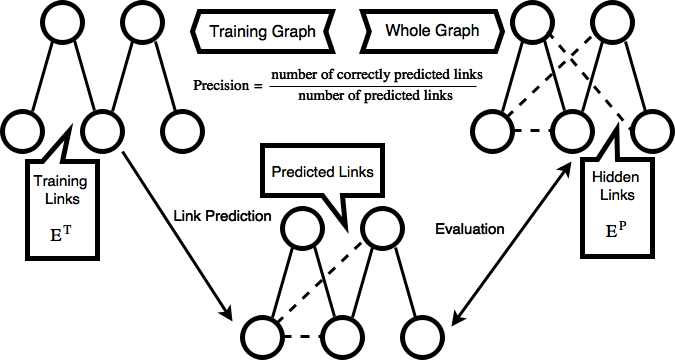
\includegraphics[scale = 0.5]{\main/img/evaluation.png}
\caption{Evaluation procedures: Hidden true links are compared to predicted links. How many predicted links where truly there?}
\label{example}
\end{figure}


\subsection{Local Community Detection for Uncertain Networks}
As mentioned in the introduction, local communities are densely-connected node sets which are discovered and evaluated based only on local information. The task of local community detection aims to find a local community for a certain start node. Clauset, Jiyang and Wu proposed local community detection problem settings for certain networks in \cite{clauset2005finding,chen2009detecting,wu2012local}. Here, we reiterate them in the context of uncertain networks.

Suppose that in an undirected network $\mathcal{G}$, we start with one node and we know all its possible neighbors and the possibilities of edge existence between the start node and all possible neighbors. Note we use ``possible" here because there exists uncertainty in the existence of edges between start node and neighbors. The possibility is in the range of (0,1]. We use $\mathcal{D}$ to denote the known local community of the graph (for the start node). This necessarily implies that we also have limited information for another shell node set $\mathcal{S}$, which contains nodes that are possible neighbors of nodes in $\mathcal{D}$ but do not belong to $\mathcal{D}$ (note ``limited" means nodes in $\mathcal{S}$ may also have other possible neighbors that are not in $\mathcal{D}$, but we do not know this information until we visit them). In such circumstances, the only way to gain additional information about the network $\mathcal{G}$ is to visit possible neighbor nodes $s_i$ of $\mathcal{D}$ (where $s_i\in \mathcal{S}$) and obtain the possible neighbors of $s_i$ and the possibilities of edge existence between $s_i$ and its neighbors. As a result, $s_i$ is removed from $S$ and becomes a member of $\mathcal{D}$ while additional nodes of $s_i$ may be added to $\mathcal{S}$. Furthermore, nodes in $\mathcal{D}$ can be split into two groups: the core node set $\mathcal{C}$, where any node $c_i\in \mathcal{C}$ has no outward links, which means all possible neighbors of $c_i$ belong to $\mathcal{D}$; and the boundary node set $\mathcal{B}$, where any node $b_i\in \mathcal{B}$ have at least one possible neighbor in $\mathcal{S}$. Figure \ref{Local_Community_Definition} shows node sets $\mathcal{D}$, $\mathcal{S}$, $\mathcal{C}$ and $\mathcal{B}$ in a network.

\begin{figure}
\centering
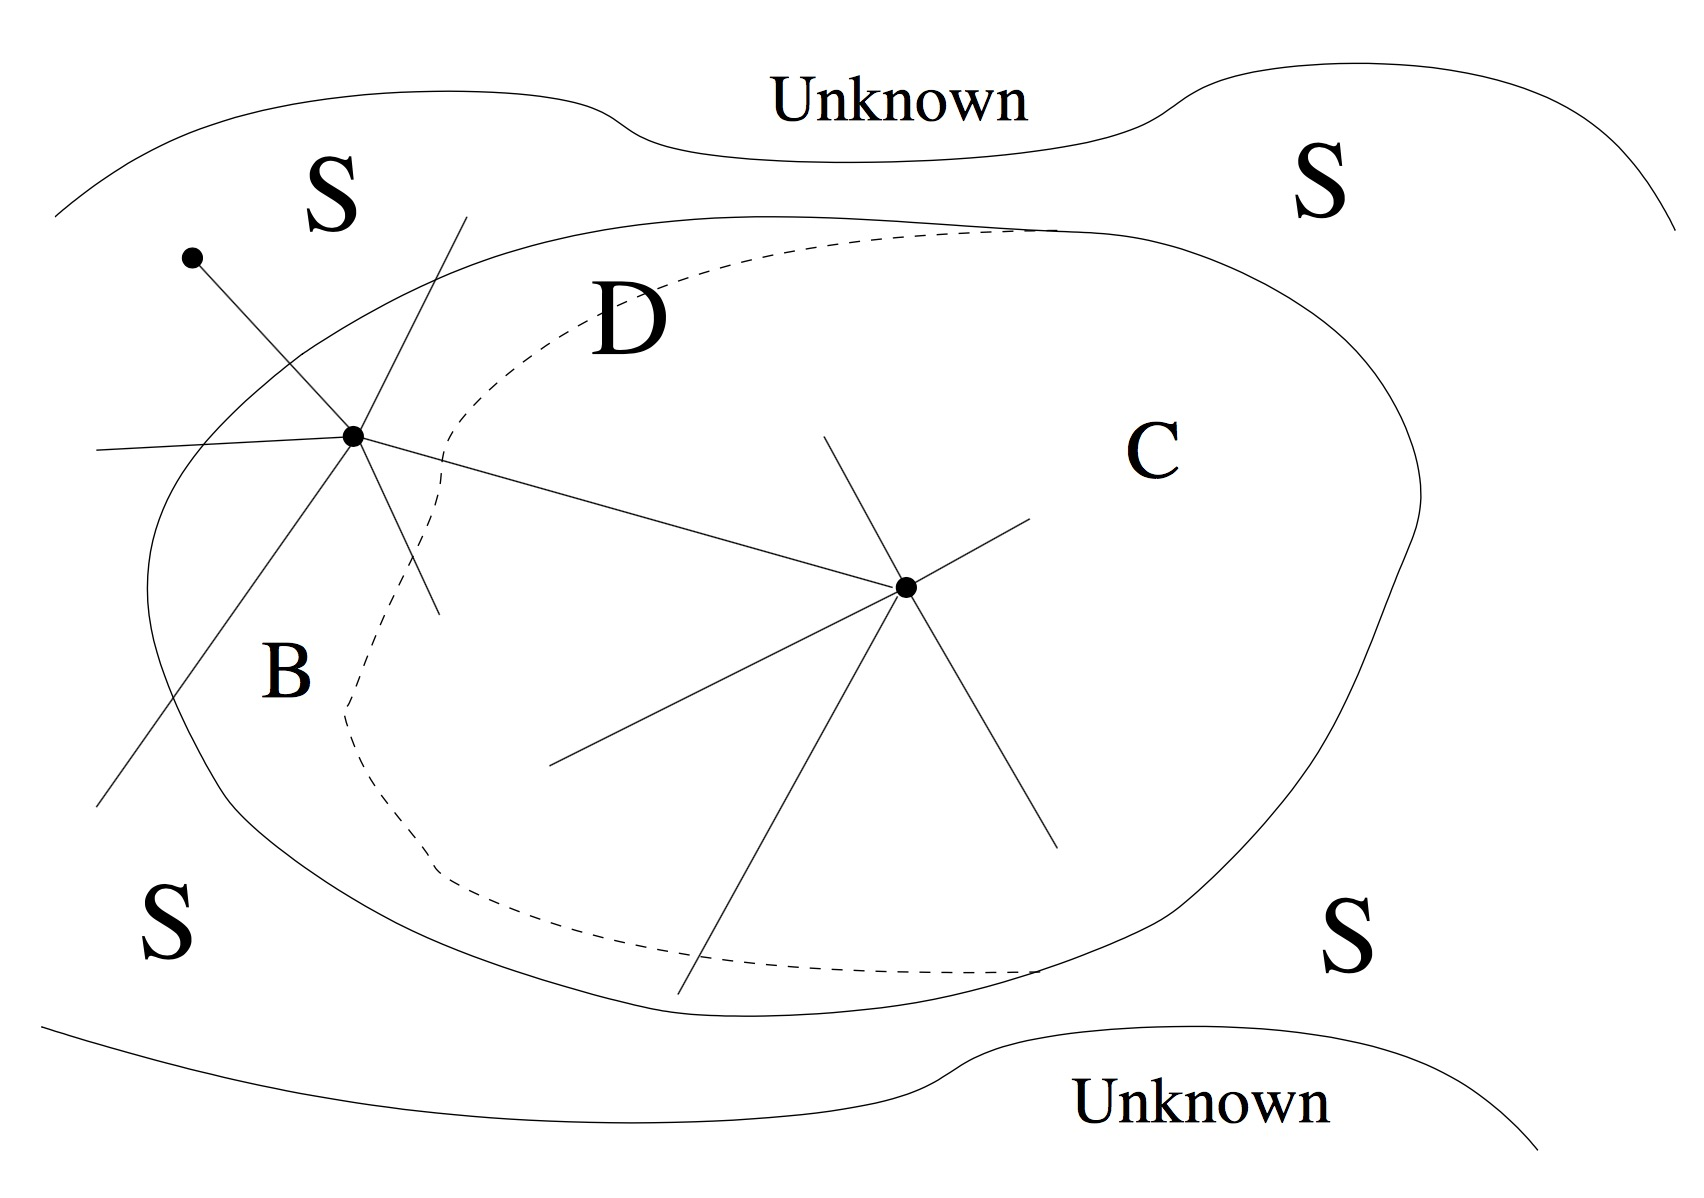
\includegraphics[scale = 0.12]{\main/img/localCommunityDefinition.jpeg}
\caption{Local Community Definition}
\label{Local_Community_Definition}
\end{figure}

\subsection{Centrality Measures for Uncertain Networks}
Centrality measures are proposed to capture the relative importance of nodes in networks. In the context of uncertain networks, some fundamental requirements of proposing uncertain version of centrality measures should be noticed: (1) The uncertain version of centrality measures should also be able to rank nodes properly; (2) A certain network can be regarded as a special case of the uncertain network, therefore, applying the uncertain version and the original version of centrality measures on the same certain graph should get the same ranking results.

\section{Thesis Contributions}

\begin{enumerate}
\item[$\bullet$] \textbf{Uncertain Network Generator:}  Due to the very limited publicly available uncertain network datasets, we put forward a way to generate uncertain networks.
\item[$\bullet$] \textbf{Link Prediction:}  We propose the uncertain version of the popular common-neighbors-based metrics and efficient algorithms to calculate them. The metrics are developed by considering all possible worlds generated by the uncertain network.
\item[$\bullet$] \textbf{Local Community Detection:} We propose a way to convert the uncertain community detection problem into the deterministic scenario. Then we illustrate with an example that periphery nodes tend to be grouped into their neighbor communities in uncertain networks, and we propose a new measure $\mathcal{K}$ to tackle this problem.
\item[$\bullet$] \textbf{Centrality Measures:}  We propose a conceptually straightforward as well as computationally efficient way to calculate centrality in uncertain networks. The method can be applied to not only unweighted uncertain networks, but also weighted uncertain networks.

\end{enumerate}

\section{Organization of the Thesis}

% \section{Cross-Referencing}\label{sec:crossRef}

% Cross-references between child documents are possible using the
% \href{https://ctan.org/pkg/xr-hyper}{\texttt{xr-hyper}} package.

% \newpage

% Text on a new page, to test top margin size.

% A sample equation \eqref{eq:test} follows:

% \begin{equation}
% y = \frac{1}{x^2} + 4 \label{eq:test}
% \end{equation}

% A sample table, Table \ref{tab:test}:

% \begin{table}[h]
%     \centering
%     \begin{tabulary}{0.75\textwidth}{r|L}
%     \textbf{Non-wrapping column} & \textbf{Wrapping column} \\ \hline
%     This is an ordinary column & This is a balanced-width column, where text will wrap
%     \end{tabulary}
%     \caption[A sample table] {A sample table created using the \href{https://ctan.org/pkg/tabulary}{\texttt{tabulary}} package}
%     \label{tab:test}
% \end{table}

\end{document}